\chapter{Simulation}\label{chap:Simulation}

Um die Ergebnisse der Vorauslegung zu vergleichen wurde mithilfe ANSYS Fluent das Verhalten des reinen \ac{pcm} und der
aerodynamischen Aufheizung simuliert.

\section{PCM}\label{sec:sim_pcm}

Für die Simulation des \ac{pcm} wurde die in Abbildung~\ref{fig:pcm_struktur} dargestellte Struktur stark vereinfacht,
um sie trotz mangelnder Rechenressourcen simulieren zu können. Zuerst wurde das \ac{pcm} in der Symmetrieebene
zu einem zweidimensionalen Problem vereinfacht. Im nächsten Schritt wurde nur die mittlere Zelle aus der Ebene unter der Annahme,
dass das System symmetrisch ist, ausgewählt. Im letzten Schritt wurde die Zelle nochmal aufgrund von Symmetrie gespalten.
Die Domäne kann man in Abbildung~\ref{fig:pcm_struktur} überlagert sehen.
Anschließend wurde in ANSYS Mechanical das Mesh (Gitternetz) vollständig aus Tetraeder-Elementen erzeugt, wobei die Elementgröße so gewählt
wurde, dass die Aluminiumwände über 1-2 Zellschichten aufgelöst sind. In dem Mesh aus Abbildung~\ref{fig:pcm_mesh} ist das \ac{pcm} in schwarz und das Aluminium
in rot dargestellt. Jeweils an der linken und rechten Kante wurde aufgrund der anliegenden Zelle bzw. Spiegelung der Zelle eine
Symmetrie-Randbedingung gewählt. Diese Randbedingung reduziert sich beim Aluminium auf eine adiabatische Wand; beim \ac{pcm}
ist diese Randbedingung adiabat mit einer Slip-Bedingung (kein Normalfluss, keine Schubspannung). Die untere Kante wurde als Wärmequelle angelegt und die obere Kante als adiabatische Wand.

Die Wärmequelle ergibt sich aus der Seitenfläche der \ac{pcm}-Struktur, bestimmt in Kapitel~\ref{sec:pcm}, und dem Avionik-Wärmestrom zu
$\frac{\SI{40}{\watt}}{\left(\SI{6,749}{\centi\meter}\right)^2} = \SI{8782}{\watt\per\meter\squared}$.
Da ANSYS Fluent bei zweidimensionalen Simulationen eine Referenztiefe von \SI{1}{m} verwendet, konnte der spezifische Wärmestrom
der Quelle direkt verwendet werden.
Die thermophysikalischen Eigenschaften von n-Eicosan sind aufgeführt in Tabelle~\ref{tab:eicosane_data}.
Das temperaturabhängige Verhalten der spezifischen Wärmekapazität, wie es in der \ac{udf} modelliert ist, kann den Abbildungen~\ref{fig:pcm_effective_cp} und \ref{fig:pcm_sensible_cp}
entnommen werden. In Abbildung~\ref{fig:pcm_effective_cp} ist der Anstieg der spezifischen Wärmekapazität infolge der
Schmelzenthalpie über die Mushy-Zone (Schmelzbereich) zu erkennen. Abbildung~\ref{fig:pcm_sensible_cp} zeigt den Verlauf der sensiblen spezifische Wärmekapazität
von der Feststoffphase, über die Mushy-Zone und in die Flüssigphase.

\begin{figure}[!htb]
    \centering
    \begin{subfigure}[t]{0.7\textwidth}
        \centering
        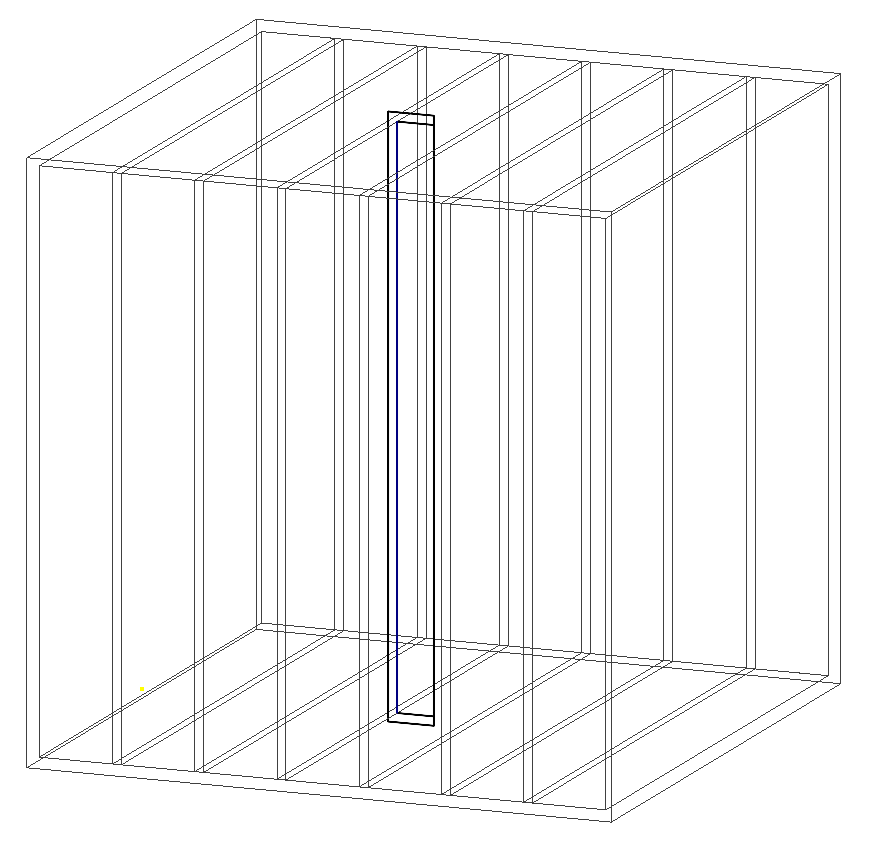
\includegraphics[height=9cm]{ansyspost/pcm/40WPCM_struktur_neu.png}
        \caption{\acs{pcm}-Struktur Drahtmodell mit vereinfachter Domäne}\label{fig:pcm_struktur}
    \end{subfigure}
    \hfill
    \begin{subfigure}[t]{0.15\textwidth}
        \centering
        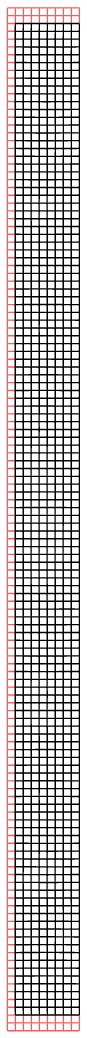
\includegraphics[height=9cm]{ansyspost/pcm/2DPCM_mesh.png}
        \caption{\acs{pcm} Mesh der vereinfachten Domäne}\label{fig:pcm_mesh}
    \end{subfigure}
    \caption{\acs{pcm}-Struktur und vereinfachtes Mesh.}\label{fig:pcm_geometrien}
\end{figure}

\begin{table}[H]

  \centering
  \caption{Stoffdaten für n-Eicosan.}\label{tab:eicosane_data}

  \begin{tabular}{lll}

    \toprule[1pt]
    Solidus Temperatur & $T_{\text{solidus}}$ & \SI{309}{\kelvin}~\cite{NIST} \\

    \midrule[0.5pt]
    Liquidus Temperatur & $T_{\text{liquidus}}$ & \SI{311}{\kelvin}~\cite{NIST} \\

    \midrule[0.5pt]
    Spezifische Wärmekapazität bei\\konstantem Druck der\\Flüssigphase & $c_{p,\text{liquid}}$ & \SI{2350,05}{\joule\per\kilogram\per\kelvin}~\cite{NIST} \\

    \midrule[0.5pt]
    Spezifische Wärmekapazität bei\\konstantem Druck der\\Feststoffphase & $c_{p,\text{solid}}$ & \SI{2132,4}{\joule\per\kilogram\per\kelvin}~\cite{NIST} \\

    \midrule[0.5pt]
    Dichte der Flüssigphase & $\rho_{\text{solid}}$ & \SI{769}{\kilogram\per\cubic\meter}~\cite{Nazarychev-2022} \\

    \midrule[0.5pt]
    Dichte der Feststoffphase & $\rho_{\text{liquid}}$ & \SI{910}{\kilogram\per\cubic\meter}~\cite{Nazarychev-2022} \\

    \midrule[0.5pt]
    Wärmeleitfähigkeit der Flüssigphase & $\lambda_{\text{liquid}}$ & \SI{0,1505}{\watt\per\meter\per\kelvin}~\cite{Benbrika-2020} \\

    \midrule[0.5pt]
    Wärmeleitfähigkeit der Feststoffphase & $\lambda_{\text{solid}}$ & \SI{0,4248}{\watt\per\meter\per\kelvin}~\cite{Stryker-1990} \\

    \midrule[0.5pt]
    Wärmeausdehnungskoeffizient & $\beta$ & \SI{0,0009}{\per\kelvin}~\cite{Benbrika-2020} \\

    \midrule[0.5pt]
    Spezifische Schmelzenthalpie & $h_{\text{fus}}$ & \SI{240998,86}{\joule\per\kilogram}~\cite{NIST} \\

    \bottomrule[1pt]
  \end{tabular}
\end{table}

\begin{figure}[H]
  \centering
  \includegraphics[width=\linewidth]{../../Code/eicosane_cpvst_total.pdf}
  \caption{Effektive spezifische Wärmekapazität von n-Eicosan.}\label{fig:pcm_effective_cp}
\end{figure}

\begin{figure}[H]
  \centering
  \includegraphics[width=\linewidth]{../../Code/eicosane_cpvst_sensible.pdf}
  \caption{Sensible spezifische Wärmekapazität von n-Eicosan.}\label{fig:pcm_sensible_cp}
\end{figure}

Die Simulation wurde mit dem pressure-based solver~\cite{akamcae-udf} als transiente Simulation über 120000 Zeitschritte mit einer Zeitschrittgröße von \SI{0,01}{\second} durchgeführt,
um die vollständige Flugdauer mit \SI{1200}{\second} zu simulieren.
Des Weiteren wurde das Energiemodell eingeschaltet~\cite{akamcae-udf}, das Viskositätsmodell als Laminar angenommen~\cite{akamcae-udf} und das Phasenwechselmodell aktiviert~\cite{akamcae-udf}.
Neben den bereits erläuterten \ac{pcm}-Eigenschaften wurde für das Aluminium eine Dichte von $\rho = \SI{2719}{\kilogram\per\meter\cubed}$,
eine spezifische Wärmekapazität von $c_p = \SI{871}{\joule\per\kilogram\kelvin}$ und eine Wärmeleitfähigkeit von $\lambda = \SI{202,4}{\watt\per\meter\kelvin}$
eingestellt.

Abbildung~\ref{fig:approximierte_beschleunigung} zeigt das Beschleunigungsprofil, das in der Simulation verwendet wurde. Zu beachten
ist, dass Beschleunigungsspitzen durch den Fallschirm, wie sie in~\ref{fig:acceleration_over_time} gesehen
werden können, ignoriert werden, da diese aus mangelhafter Genauigkeit der Fallschirmmodellierung resultieren.

\begin{figure}
  \centering
  \includegraphics[width=\linewidth]{../../Code/approximate_acceleration_over_time.pdf}
  \caption{Approximiertes Beschleunigungsprofil.}\label{fig:approximierte_beschleunigung}
\end{figure}

Da der ANSYS Fluent transient table (native Funktion für transiente Randbedingungen mit Profilen) keine transiente Gravitation
unterstützt, wurde diese und die globale Beschleunigung deaktiviert.
Stattdessen wurde die Beschleunigung über den Quellterm der Boussinesq-Approximation in der \ac{udf} implementiert. Die Funktion ist im
Programmcode~\ref{lst:udf_bossinesque} zu sehen. Der vollständige Programmcode mit allen temperaturabhängigen Funktionen aus Kapitel \ref{sec:pcm_grundlagen} ist in \ref{lst:udf_rest} zu sehen.

Als Kopplungsschema wurde SIMPLE verwendet~\cite{akamcae-udf}. Für die Gradienten least-squares cell-based~\cite{akamcae-udf}, für Druck second-order~\cite{akamcae-udf} und für Impuls und Energie
second-order-upwind~\cite{akamcae-udf}. Die Unterrelaxationsfaktoren wurden durch experimentelle Ermittlung anhand der Residuen zu 0,3 für Druck, 1 für Dichte
und Körperkräfte, 0,5 für Impuls und 0,9 für sowohl Flüssigkeitsanteil als auch Energie gewählt.

\begin{figure}
    \centering

    % Left figure
    \begin{minipage}[t]{0.485\textwidth}
        \centering
        \setlength{\tabcolsep}{1pt} % reduce subfigure spacing
        % Legend vertically centered & with extra space to right
        \begin{subfigure}[t]{0.16\textwidth}
            \centering
            \raisebox{0.7\height}{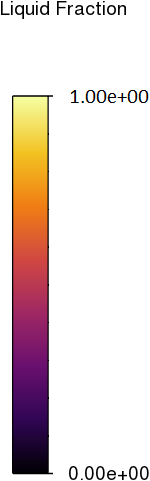
\includegraphics[height=0.2\textheight]{ansyspost/pcm/liquid-fraction-legend.png}}
        \end{subfigure}%
        \hspace{2mm}% extra space between legend and first image
        \begin{subfigure}[t]{0.2\textwidth}
            \centering
            
\includegraphics[height=0.5\textheight]{ansyspost/pcm/liquid-fraction-300.png}
            \caption{\SI{300}{\second}}\label{fig:liquid_fraction_300}
        \end{subfigure}%
        \begin{subfigure}[t]{0.2\textwidth}
            \centering
            
\includegraphics[height=0.5\textheight]{ansyspost/pcm/liquid-fraction-600.png}
            \caption{\SI{600}{\second}}\label{fig:liquid_fraction_600}
        \end{subfigure}%
        \begin{subfigure}[t]{0.2\textwidth}
            \centering
            
\includegraphics[height=0.5\textheight]{ansyspost/pcm/liquid-fraction-900.png}
            \caption{\SI{900}{\second}}\label{fig:liquid_fraction_900}
        \end{subfigure}%
        \begin{subfigure}[t]{0.2\textwidth}
            \centering
            
\includegraphics[height=0.5\textheight]{ansyspost/pcm/liquid-fraction-1200.png}
            \caption{\SI{1200}{\second}}\label{fig:liquid_fraction_1200}
        \end{subfigure}
        \caption{Flüssigkeitsanteil Konturen. Die Legende bezieht sich auf~\ref{fig:liquid_fraction_1200}}
        \label{fig:liquid_frac_kontur}
    \end{minipage}
    \hspace{2mm} % small horizontal space
    % Right figure
    \begin{minipage}[t]{0.485\textwidth}
        \centering
        \begin{subfigure}[t]{0.16\textwidth}
            \centering
            \raisebox{0.7\height}{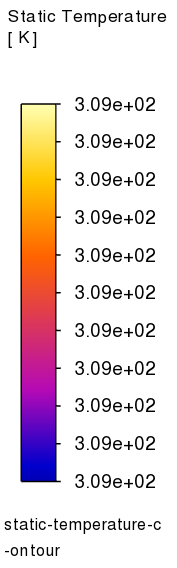
\includegraphics[height=0.2\textheight]{ansyspost/pcm/temperature-legend.png}}
        \end{subfigure}%
        \hspace{2mm}% extra space between legend and first image
        \begin{subfigure}[t]{0.2\textwidth}
            \centering
            
\includegraphics[height=0.5\textheight]{ansyspost/pcm/static-temperature-300.png}
            \caption{\SI{300}{\second}}\label{fig:temperatur_300}
        \end{subfigure}%
        \begin{subfigure}[t]{0.2\textwidth}
            \centering
            
\includegraphics[height=0.5\textheight]{ansyspost/pcm/static-temperature-600.png}
            \caption{\SI{600}{\second}}\label{fig:temperatur_600}
        \end{subfigure}%
        \begin{subfigure}[t]{0.2\textwidth}
            \centering
            
\includegraphics[height=0.5\textheight]{ansyspost/pcm/static-temperature-900.png}
            \caption{\SI{900}{\second}}\label{fig:temperatur_900}
        \end{subfigure}%
        \begin{subfigure}[t]{0.2\textwidth}
            \centering
            
\includegraphics[height=0.5\textheight]{ansyspost/pcm/static-temperature-1200.png}
            \caption{\SI{1200}{\second}}\label{fig:temperatur_1200}
        \end{subfigure}
        \caption{Konturen der statischen Temperatur. Die Legende bezieht sich auf~\ref{fig:temperatur_1200}.}
        \label{fig:static_temperature_kontur}
    \end{minipage}

\end{figure}

In Abbildung~\ref{fig:liquid_frac_kontur} und \ref{fig:static_temperature_kontur} kann man jeweils die Lösung des Flüssigkeitsanteils
und der statischen Temperatur zu mehreren Zeitschritten sehen. Man kann dort deutlich erkennen, wie das \ac{pcm} von der Wärmequelle aus
schmilzt. Besonders an der Aluminiumlamelle bildet sich eine beschleunigte Konvektion, die jedoch nach unten fließt und durch das aufsteigende
\ac{pcm} in der Mitte der Zelle angetrieben wird. Im Vektorfeld~\ref{fig:pcm_vectoren_stitched} kann man den dadurch entstandenen Wirbel sehen.
Die Wirbelentwicklung in weiteren Zeitschritten zeigt Abbildung~\ref{fig:pcm_velocity_vektoren_kontur}. Die Legenden beziehen sich immer auf den letzten
Zeitschritt, da der maximale Flüssigkeitsanteil und die maximale Temperatur dort am höchsten sind.

\begin{lstlisting}[language=C, float, caption={Boussinesq-Approximation des Auftriebs im \ac{pcm} in der \ac{udf} eicosane.c}, label={lst:udf_bossinesque}]
//Y-momentum source
DEFINE_SOURCE(Boussinesq_momentum_source,cell,thread,dS,eqn)
{
	double Temp, source, acc;
	Temp=C_T(cell,thread);

	double t = CURRENT_TIME;

	if (t < 20)
		acc = 34.81;
	else if (t < 50)
		acc = 109.81;
	else if (t < 150)
		acc = 19.62;
	else
		acc = 9.81;

	source=-Rol_pcm*acc*TEC*(Temp-Tr);  //negative for -Y down
	dS[eqn]=-Rol_pcm*acc*TEC; 			//negative for -Y down
	return source;
}
\end{lstlisting}

\begin{figure}[H]
  \centering
  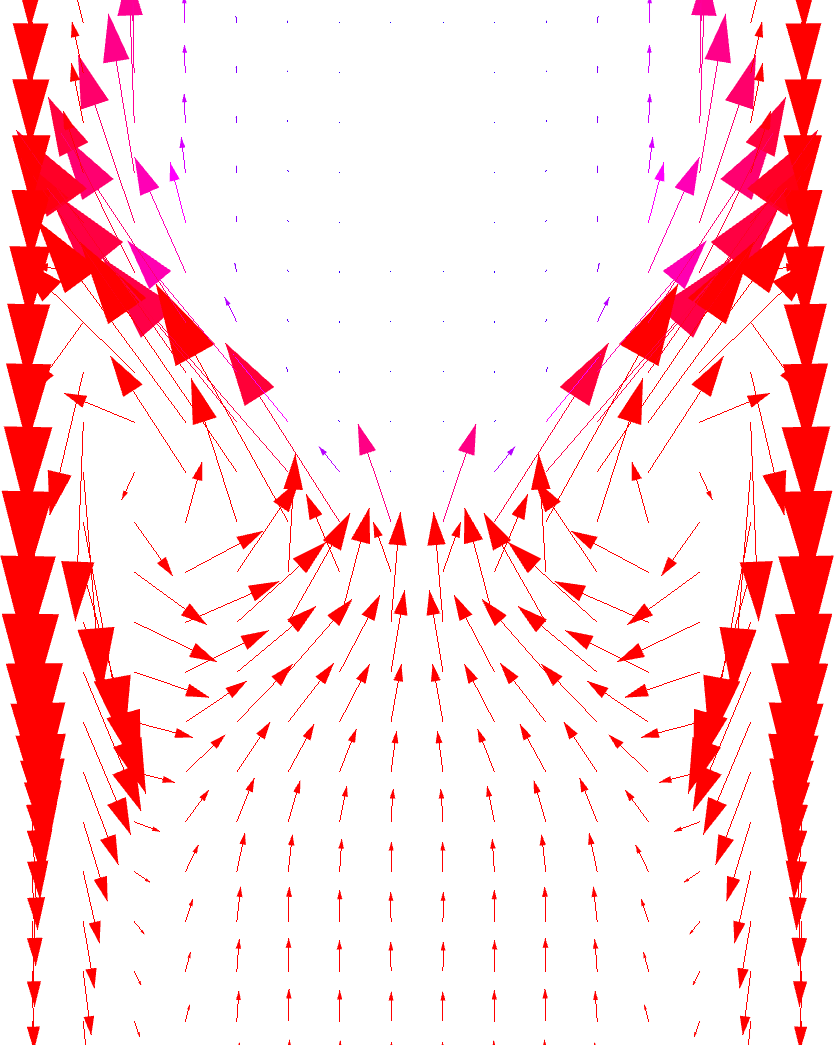
\includegraphics[height=0.4\textheight]{ansyspost/pcm/velocity-vector-close-stitched-900.png}
  \caption{Geschwindigkeitsvektoren der Konvektionswirbel einer durch Nachbearbeitung vervollständigten Zelle
  bei \SI{900}{\second}. Darstellung der weiteren Zeitschritte ist in Abbildung~\ref{fig:pcm_velocity_vektoren_kontur} zu finden.}\label{fig:pcm_vectoren_stitched}
\end{figure}

Besonders interessant ist, dass, wie in Abbildung~\ref{fig:static_temperature_kontur} zu erkennen ist, die Temperatur an der Quelle auf bis zu \SI{336}{\kelvin}
steigt. Demnach würde mittels der thermalen Schnittstelle aus Kapitel~\ref{sec:thermale_schnittstelle} die Gehäusetemperatur der Avionik-Bauteile mit
$T_C = \SI{384,17}{\kelvin}$ über die zulässige Temperatur steigen.

\section{Aerodynamische Aufheizung}\label{sec:sim_aerodynamisch}

Die Simulationen der aerodynamischen Aufheizung wurden als stationäre Simulationen mit dem density-based solver durchgeführt.
Aufgrund der Ähnlichkeit wurden diese stark an der Masterarbeit zur aerodynamischen Analyse des vorherigen
\ac{hyend} Projekts N2ORTH von Hugh Irving~\cite{Irving-2021} orientiert.
Als Viskositätsmodell wurde SST k-$\omega$~\cite{Irving-2021} gewählt und das Energiemodell aktiviert~\cite{Irving-2021}.
Die Luft wurde als ideales Gas~\cite{Irving-2021} mit einer spezifischen Wärmekapazität von \SI{1006,43}{\joule\per\kilogram\kelvin},
einer Wärmeleitfähigkeit von \SI{0,0242}{\watt\per\meter\kelvin}, einer dynamischen Viskosität von \SI{1,7894e-5}{\kilogram\per\meter\second}
und einer molekularen Masse von \SI{28,966}{\kilogram\per\kilo\mole} modelliert.
Weiterhin wurde für Gradienten green-gauss cell-based und für Fluss, Turbulente kinetische Energie sowie spezifische Dissipationsrate second-order upwind verwendet.
Für Formulierung wurde implicit und für den Flusstyp Roe-FDS gewählt.

Die Umströmungssimulationen der Rakete wurden an \ac{maxq} orientiert, dem Zeitpunkt des maximalen dynamische Drucks auf der Rakete.
Den Verlauf des dynamischen Drucks kann man Abbildung~\ref{fig:dynp_over_time} entnehmen.
Dieser Punkt wird als Richtwert für die aerodynamische Aufheizung angenommen, da er unabhängig von der Vorauslegung ist und somit Ungenauigkeiten dort getroffener Annahmen vermieden werden.

Um ein Profil der aerodynamischen Aufheizung bilden zu können wurde jeweils eine Simulation bei \ac{maxq}, \ac{maxq}-\SI{10}{\second},
\ac{maxq}+\SI{10}{\second} und \ac{maxq}+\SI{20}{\second} durchgeführt. Die den Punkten entsprechenden Flugzustände können Tabelle~\ref{tab:simulation_flugzustand} entnommen werden.

\begin{table}[H]
  \centering
  \caption{Flugzustände der vier Simulationen zur aerodynamischen Aufheizung.}\label{tab:simulation_flugzustand}

  \begin{tabular}{lrrrrrr}
    \toprule[1pt]
    Zustand & $t$ [s] & $h$ [m] & $U$ [m/s] & $T$ [°C] & $p$ [hPa] & $\rho$ [kg/m³] \\
    \midrule[0.5pt]
    \ac{maxq} $-10$ s    & 18,691 & 4274,387  & 461,355  & -12,784 & 594,935 & 0,796 \\
    \ac{maxq}            & 28,691 & 10244,138 & 750,704  & -51,587 & 254,783 & 0,401 \\
    \ac{maxq} $+10$ s    & 38,691 & 19758,652 & 1189,968 & -56,500 & 56,930  & 0,092 \\
    \ac{maxq} $+20$ s    & 48,700 & 32439,616 & 1393,377 & -43,269 & 8,136   & 0,012 \\
    \bottomrule[1pt]
  \end{tabular}
\end{table}

Bei dieser Simulation wurde aufgrund der Rotationssymmetrie der Rakete im relevanten Bereich oberhalb der Finnen eine zweidimensionale Simulation der halben Rakete durchgeführt.
Das Mesh der Domäne wurde in ANSYS Mechanical vollständig aus Tetraeder-Elementen erstellt und ist samt Randbedingungen und Partitionen der Parallelisierung in Abbildung~\ref{fig:aussenstroemung_mesh} dargestellt.
Dort sind die blauen Pfeile auf der linken Seite der velocity-inlet und die roten Pfeile auf der rechten Seite der pressure-outlet.
Die übrigen Ränder der Domäne, abzüglich der Nase und Hülle der Rakete, in gelb sind Symmetrie-Randbedingungen.
Die Nase selbst wurde als adiabatische Wand mit no-slip modelliert und das Hüllensegment als isotherm mit no-slip aufgrund des \ac{pcm} mit $T_w = \SI{310}{\kelvin}$ (Schmelzpunkt des n-Eicosan).

Um die Anforderung der Gleichung~\ref{eq:yplus} mit $y^+ \leq 1$ zu erfüllen, wurden Inflationsschichten an der Wand eingefügt, die in Abbildung~\ref{fig:aussenstroemung_mesh_inflationlayers}
zu sehen sind. Zur Berechnung der Höhe der ersten Zellschicht wurde der Flugzustand bei \ac{maxq} verwendet.
Zuerst muss Gleichung~\ref{eq:dynamische_viskositaet} verwendet werden, um die dynamische Viskosität zu berechnen:

\begin{equation*}
  \eta_\mathrm{max Q} = \SI{18,27e-6}{\pascal\second} \frac{\SI{291,15}{\kelvin} + \SI{120}{\kelvin}}{\SI{221,563}{\kelvin} + \SI{120}{\kelvin}} {\left( \frac{\SI{221,563}{\kelvin}}{\SI{291,15}{\kelvin}} \right)}^{\frac{3}{2}} \approx \SI{1,45e-5}{\pascal\second}
\end{equation*}

Damit wird als nächstes die lokale Reynolds-Zahl in der Mitte des Radiators berechnet. Die Konturlänge bis zu dem Mittelpunkt des Radiators ist wie in Kapitel~\ref{sec:pcm_radiator_hybrid} \SI{1,074}{\meter}:

\begin{equation*}
  Re_{\mathrm{maxQ}} = \frac{\SI{750,704}{\meter\per\second}\,\SI{0,401}{\kilogram\per\meter\cubed}\,\SI{1,074}{\meter}}{\SI{1,45e-5}{\pascal\second}} \approx \SI{2,220e7}{}
\end{equation*}

Da die Reynolds-Zahl sich im turbulenten Bereich befindet, wird Gleichung \ref{eq:reibungsbeiwert_turbulent} für den Reibungsbeiwert verwendet:

\begin{equation*}
  C_f = \frac{0.0592}{\left({\SI{2,22e7}{}}_x\right)^{1/5}} \approx \SI{2,009e-3}{}
\end{equation*}

Mit Gleichung \ref{eq:schubspannung} eingesetzt in Gleichung \ref{eq:schubspannung_geschwindigkeit} ergibt sich für die Schubspannungsgeschwindigkeit:

\begin{equation*}
  u_{\tau} = \sqrt{\frac{\left(\SI{750,704}{\meter\per\second}\right)^2\,\SI{2,009e-3}{}}{2}} \approx \SI{23,793}{\meter\per\second}
\end{equation*}

\newpage

Zuletzt lässt sich dann mithilfe Gleichung~\ref{eq:yplus} die Höhe der ersten Zelle $y_1$ berechnen, indem $y^+ = 1$ gesetzt wird:

\begin{equation*}
  y_1 = \frac{y^+\,\SI{1,45e-5}{\pascal\second}}{\SI{0,401}{\kilogram\per\meter\cubed}\,\SI{23,793}{\meter\per\second}} \approx \SI{1,52e-6}{\meter}
\end{equation*}

\begin{figure}[H]
  \centering
  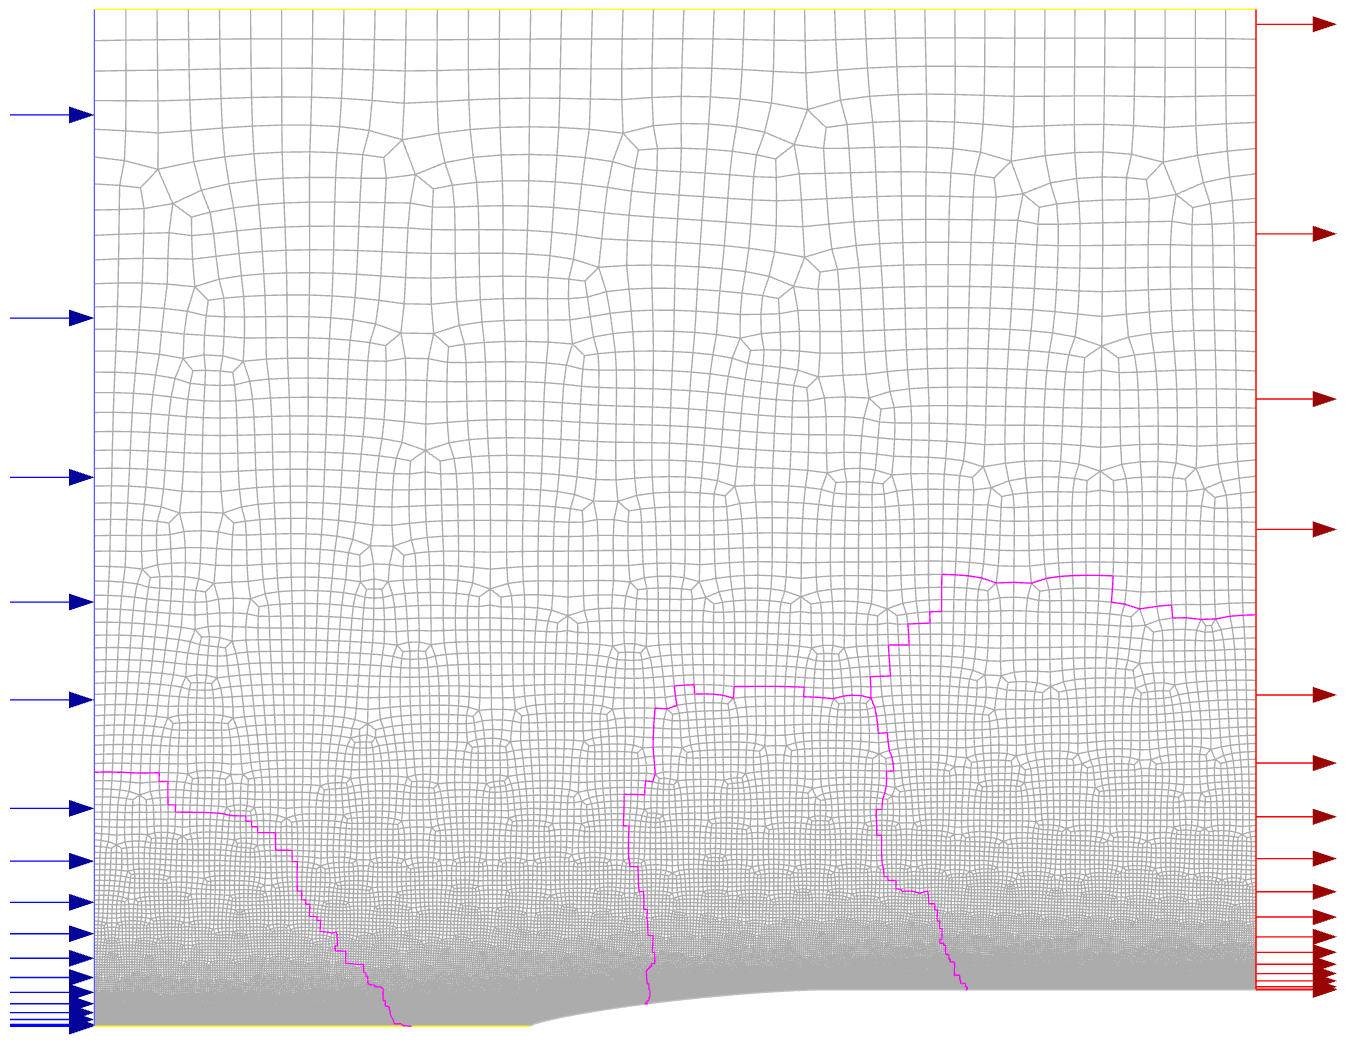
\includegraphics[width=\linewidth]{ansyspost/airflow/mesh_all.png}
  \caption{Darstellung des Setup der Außenströmungssimulation mit Meshstruktur in Grau, velocity inlet in Blau, pressure outlet in Rot, Symmetrien in Gelb und Partitionen der Parallelisierung in Lila.}\label{fig:aussenstroemung_mesh}
\end{figure}

\begin{figure}[H]
  \centering
  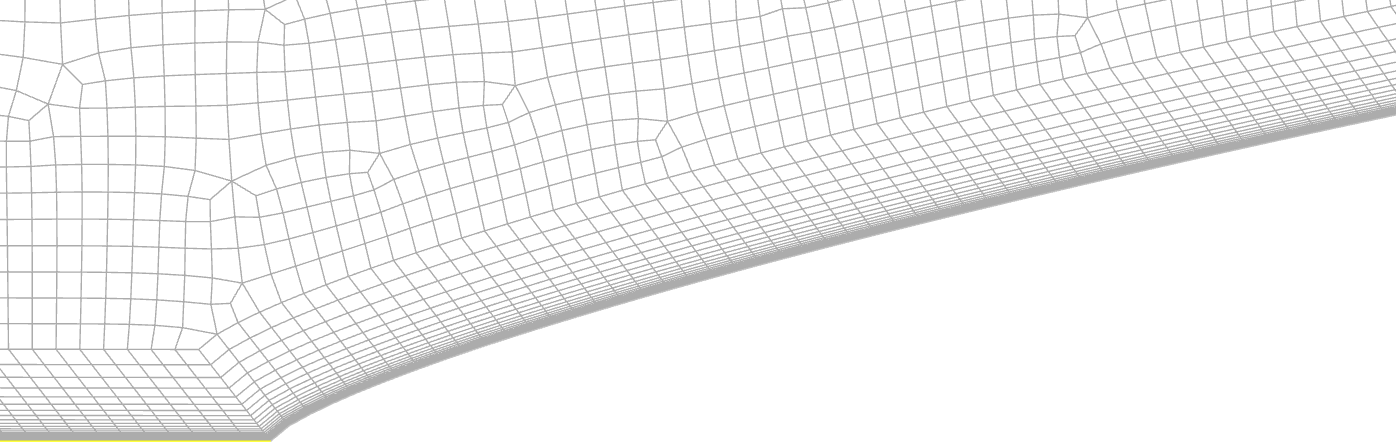
\includegraphics[width=\linewidth]{ansyspost/airflow/mesh_inflation.png}
  \caption{Inflationsschichten des Mesh an der Rakete.}\label{fig:aussenstroemung_mesh_inflationlayers}
\end{figure}

\begin{figure}[H]
  \centering
  \includegraphics[width=\linewidth]{../../Code/maxQ_compare_heatflux.pdf}
  \caption{Spezifischer Wärmestrom an der Außenhaut bei maximalem dynamischen Druck, sowie \SI{10}{s} davor, danach und \SI{20}{s} danach.}\label{fig:spezifischer_waermestrom_maxQ_simulationen}
\end{figure}

Die Simulationen wurden durchgeführt bis alle Residuen unter \SI{1e-3}{} waren und die Wärmeströme zu $\approx\SI{5}{\percent}$ konvergiert sind.
In Abbildung~\ref{fig:spezifischer_waermestrom_maxQ_simulationen} kann man den spezifischen Wärmestrom am Hüllensegment der Rakete sehen.
Die Positionsachse entspricht bei \SI{1}{\meter} dem Übergang von der Nase zum Hüllensegment. Weiterhin ist zu beachten, dass der spezifische Wärmestrom
negativ ist, wenn Wärme aus dem Fluid in die Wand übergeht. Dementsprechend kann man deutlich erkennen, dass mit der weiteren Entwicklung der Grenzschicht
der spezifische Wärmestrom sinkt.

Die Aussagekraft der spezifischen Wärmeströme über die Wand lässt sich anhand der Abbildung~\ref{fig:yplus_maxQ_simulationen} bestätigen, da die Werte von $y^+$
für alle vier Simulationen innerhalb der Bedingungen $y^+ \leq 1$ liegen.

\begin{figure}
  \centering
  \includegraphics[width=\linewidth]{../../Code/maxQ_compare_yplus.pdf}
  \caption{$y^+$ Wert an der Außenhaut bei \acs{maxq}, sowie \SI{10}{s} davor, danach und \SI{20}{s} danach.}\label{fig:yplus_maxQ_simulationen}
\end{figure}

\newpage

\begin{minipage}{\textwidth}
  Ein Vergleich der Simulationsergebnisse mit der Vorauslegung ist in Abbildung~\ref{fig:pcm_waermestrom_sim} zu sehen, in der die Abbildung~\ref{fig:pcm_waermestrom_vorauslegung} mit den
  Simulationsergebnissen überlagert wurde. Die Wärmeströme in der Mitte des Radiators sind als rote Punkte dargestellt und wurden mittels einer Gauß-Funktion und der Funktion \texttt{curve\_fit} aus dem
  Python Paket \texttt{SciPy} automatisch angepasst:

  \begin{equation*}
  f(x) = a \cdot \exp\!\left(-\frac{(x-b)^2}{2c^2}\right) + d
  \end{equation*}

  Ermittelte Parameter:
  \begin{equation*}
    a=12454028,32 \quad b=32,87 \quad c=550,50 \quad d=-12446646,16
  \end{equation*}
\end{minipage}

Die Temperatur- und Machzahlkontur der Luft kann man in Abbildung~\ref{fig:maxQ_konturen} sehen, wo der Stoß an der Nasenspitze
deutlich zu erkennen ist. Konturen der weiteren Simulationen sind den Abbildungen~\ref{fig:airflow_temp_contour_continued}
und \ref{fig:airflow_mach_contour_continued} zu entnehmen. Die Maximaltemperatur von \SI{501}{\kelvin} wird an der Spitze der Rakete erreicht.
Im Bereich des Radiators sind es $\approx \SIrange{310}{340}{\kelvin}$.

\begin{figure}
  \centering
  \includegraphics[width=\linewidth]{../../Code/pcm_radiator_hybrid_heatflux_with_sim.pdf}
  \caption{PCM Wärmestrom während Flug mit Simulationsergebnissen und Fit-Kurve.}\label{fig:pcm_waermestrom_sim}
\end{figure}

\begin{figure}
    \centering

    \begin{subfigure}{\textwidth}
        \centering
        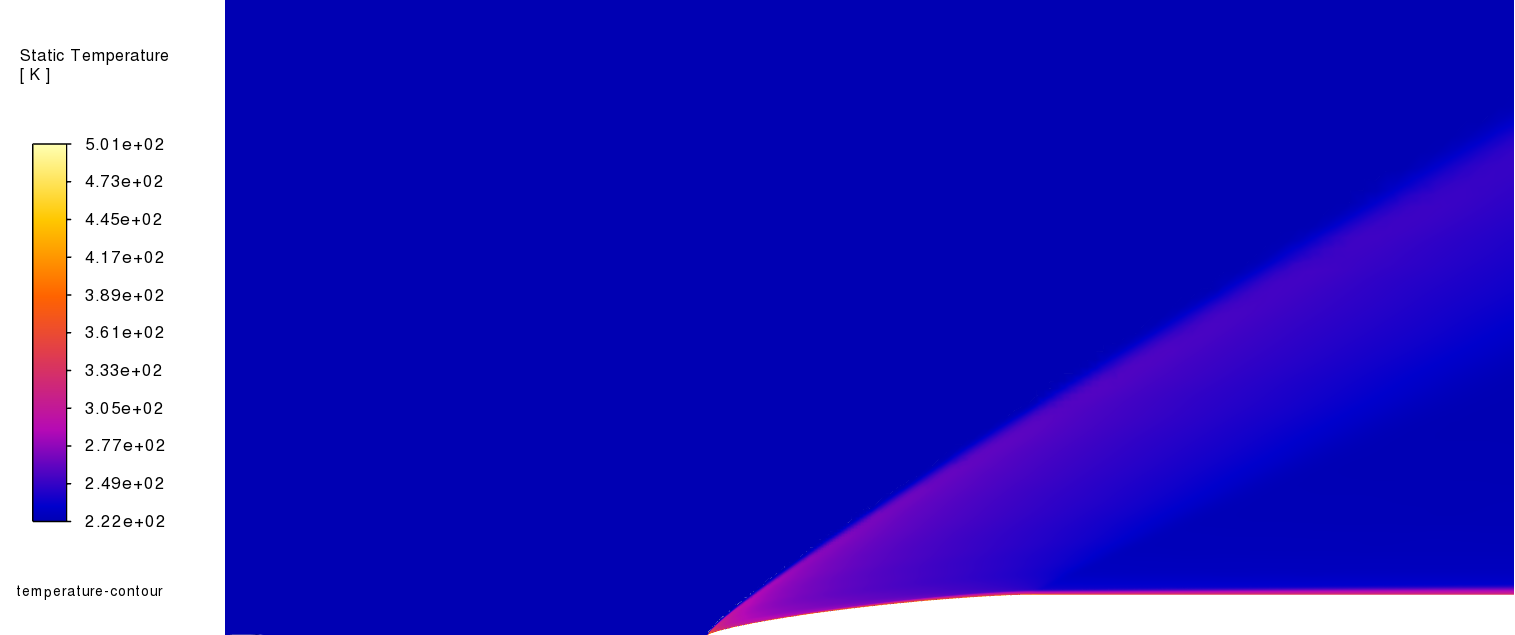
\includegraphics[height=0.23\textheight]{ansyspost/airflow/maxQ-temperature-contour.png}
        \caption{Statische Temperaturkontur der Luft.}
        \label{fig:maxQ_temp_contour}
    \end{subfigure}

    \begin{subfigure}{\textwidth}
        \centering
        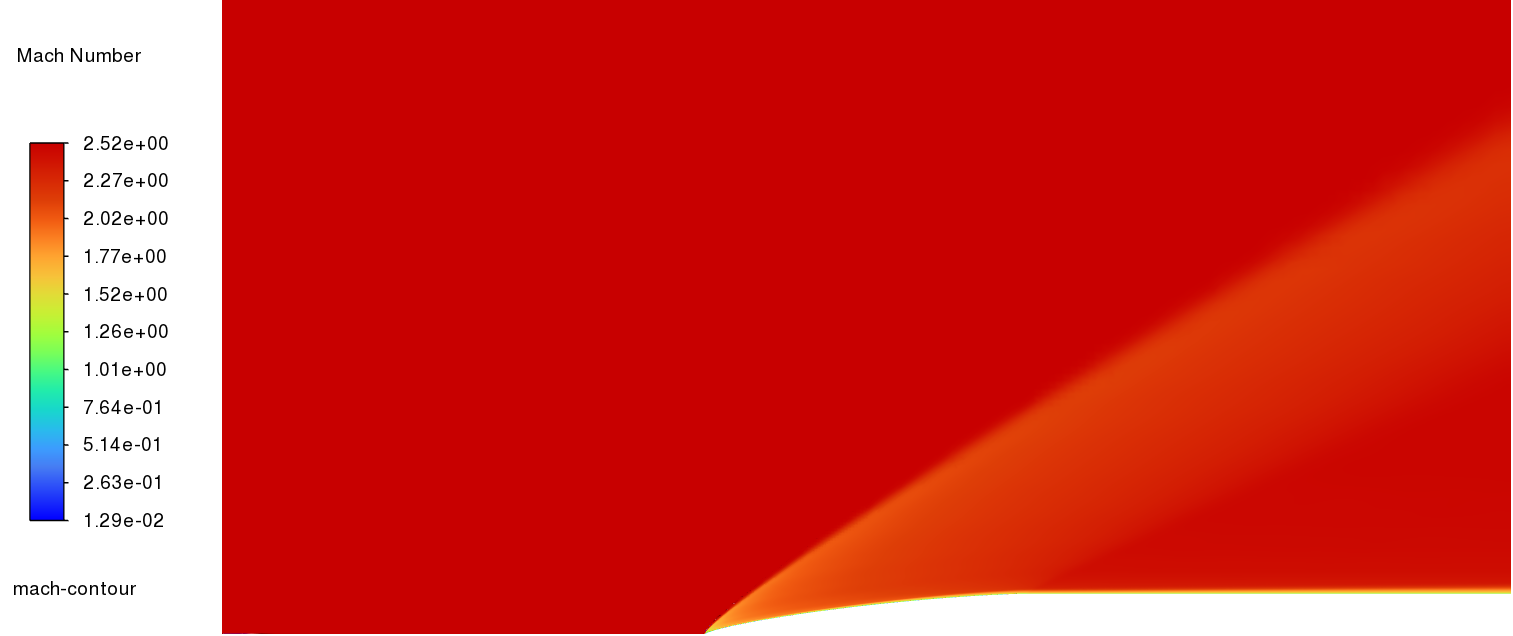
\includegraphics[height=0.23\textheight]{ansyspost/airflow/maxQ-mach-contour.png}
        \caption{Machzahlkontur der Luft.}
        \label{fig:maxQ_mach_contour}
    \end{subfigure}

    \caption{\texorpdfstring{\acs{maxq}}{max Q} Konturen der Luft}
    \label{fig:maxQ_konturen}
\end{figure}